\chapter[][3D Elastic Case]{The spectral functions method for 3D elastic wave diffraction by a stress-free wedge}
\label{chap-3D}

\section*{Introduction}

\section{Problem statement}

\begin{figure}[h]
\centering
	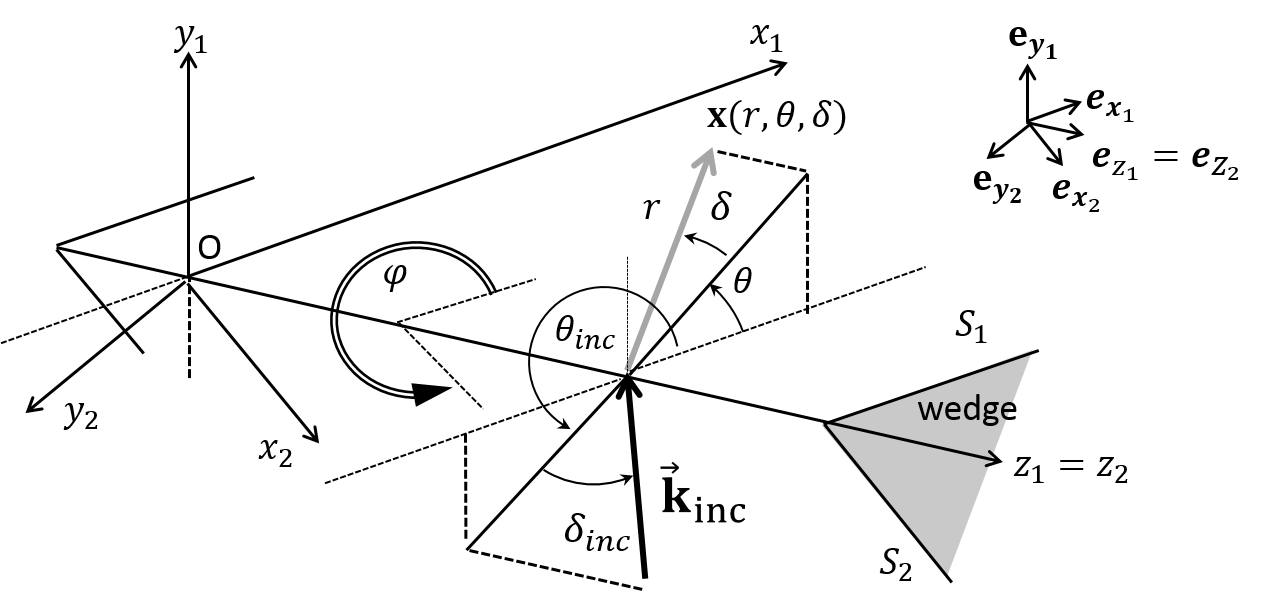
\includegraphics[width=\textwidth]{images/chapter4/wedge_3D.png}
\caption{Geometry of the problem}
\label{diedre_coords}
\end{figure}

Let us consider the problem of an elastic wave diffracted by a stress-free wedge delimited by faces $\mathcal{S}_1$ and $\mathcal{S}_2$. The geometry of the problem is shown on Fig.~\ref{diedre_coords}. The domain $\Omega$ is the inside of the wedge, defined by :
\begin{equation}
\Omega=\{ (r\cos \theta \cos \delta, r \sin \theta \cos \delta, r \sin \delta)\, \backslash \, \theta \in \rbrack 0, \varphi \lbrack, \, \delta \in \rbrack -\frac{\pi}{2}, \frac{\pi}{2} \lbrack \}
\end{equation}
%et sa surface
%$$ \mathcal{S}=\mathcal{S}_1 \cup \mathcal{S}_2 $$

The incident wave is a plane wave of the form
\begin{equation}
\mathbf{u}^{inc}(\mathbf{x},t)=\mathbf{A}_{\alpha}e^{i(\mathbf{k}_{\alpha}^{inc}\cdot \mathbf{x}-\omega t)}
\end{equation}
where $\mathbf{A}_{\alpha}$ is the amplitude vector of the incident wave and $\mathbf{k}_{\alpha}^{inc}$ is the incident wave vector. The type of the incident wave is denoted $\mathbf{k}_{\alpha}^{inc}$ (L for a longitudinal wave, TH for transverse horizontal and TV for transverse vertical). $(\mathbf{x}_1,\mathbf{y}_1, \mathbf{z}_1)$ is a Cartesian coordinate system associated to face $\mathcal{S}_1$. In this system, the incident wave vector is given by :
\begin{equation}
\mathbf{k}_{\alpha}^{inc}=\frac{\omega}{c_{\alpha}} \begin{pmatrix}
\cos\theta_{inc} \cos \delta_{inc} \\ \sin\theta_{inc} \cos \delta_{inc} \\
\sin \delta_{inc}
\end{pmatrix}
\end{equation}
As always, $c_L$ is the velocity of longitudinal waves and $c_T$ is the velocity of transverse waves.

The amplitude vector can be directed by three different and two-by-two orthogonal vectors, depending on the incident wave's polarization. These unit polarization vectors are noted $\hat{i}_*$, where $*=L, TH, TV$ and are given by Achenbach \cite{Achenbach} :
\begin{equation}
\hat{i}_L = \begin{pmatrix}
\cos\theta_{inc} \cos \delta_{inc} \\ \sin\theta_{inc} \cos \delta_{inc} \\
\sin \delta_{inc}
\end{pmatrix}
\hfill
\hfill
\hat{i}_{TV} = \begin{pmatrix}
-\cos\theta_{inc} \sin \delta_{inc} \\ -\sin\theta_{inc} \sin \delta_{inc} \\
\cos \delta_{inc}
\end{pmatrix}
\hfill
\hfill
\hat{i}_{TH} = \begin{pmatrix}
-\sin\theta_{inc} \\ \cos\theta_{inc} \\
0
\end{pmatrix}
\label{ivec}
\end{equation}

In all the following, vectors are expressed in the coordinate system $(\mathbf{x}_1,\mathbf{y}_1, \mathbf{z}_1)$, except when explicitly mentioned otherwise. For a homogeneous, isotropic material, the linear elasticity equation solved by the displacement field $\mathbf{u}$ is 
\begin{equation}
\underline{\mu} \Delta \mathbf{u} + (\underline{\lambda}+\underline{\mu})\nabla \nabla \mathbf{u} = \rho \frac{\partial^2 \mathbf{u}}{\partial t^2}
\label{C4:Elasticitelin}
\end{equation}
On each of the wedge faces, the displacement field verifies the zero-stress boundary conditions, expressed as :
\begin{equation}
(\underline{\lambda} \nabla \mathbf{u} .\mathbf{\mathbb{I}_3}+2\underline{\mu} \mathbf{\varepsilon} (\mathbf{u})).\mathbf{n}=0
\label{C4:stressfree}
\end{equation}
where $\mathbf{\mathbb{I}_3}$ is the identity matrix of the third order, $n$ is the inward facing normal to the wedge face ($n=\mathbf{y}_1$ on $\mathcal{S}_1$  and $n=\mathbf{y}_2$ on $\mathcal{S}_2$) and $\underline{\lambda}, \underline{\mu}$ are the Lamé coefficients of the considered elastic medium. The expression of the deformations tensor is :
\begin{equation}
\mathbf{\varepsilon}(\mathbf{u})=\frac{1}{2} \begin{pmatrix}
2\dfrac{\partial u_1}{\partial x_1} & \dfrac{\partial u_1}{\partial y_1}+\dfrac{\partial u_2}{\partial x_1}&\dfrac{\partial u_1}{\partial z}+\dfrac{\partial u_3}{\partial x_1} \\
\dfrac{\partial u_1}{\partial y_1}+\dfrac{\partial u_2}{\partial x_1}&2\dfrac{\partial u_2}{\partial y_1}&\dfrac{\partial u_2}{\partial z}+\dfrac{\partial u_3}{\partial y_1} \\
\dfrac{\partial u_1}{\partial z}+\dfrac{\partial u_3}{\partial x_1} &\dfrac{\partial u_2}{\partial z}+\dfrac{\partial u_3}{\partial y_1} & 2\dfrac{\partial u_3}{\partial z}
\end{pmatrix}
\end{equation}
Kamotski and Lebeau \cite{KamotskiLebeau} have proven existence and uniqueness of the solution to this problem in the 2D the case. We will suppose that their demonstration is still valid in the 3D case.

From hereon after, bold characters will be reserved to matrices in order to simplify notations. The solutions being time harmonic, the factor $e^{-i\omega t}$ will be implied but omitted everywhere. Furthermore, since there is no obstacle to propagation in the $z$ direction, $e^{i\frac{\omega}{c_{\alpha}}\sin\delta_{inc}z}$ is also a common factor to all the terms which appear in the solution.

The total field is written as the sum of an incident field $u^{inc}$ and a scattered field $u_0$
\begin{equation}
u=u_0+u^{inc}
\label{C4:scat}
\end{equation}

The dimensionless problem is obtained by applying the following variable change :
\begin{equation}
u_0(x,y,z)=v\left( \frac{\omega}{c_L} x, \frac{\omega}{c_L} y \right)e^{i\nu_{\alpha}\sin\delta_{\alpha}z}
\label{C4:adiming}
\end{equation}
where $\delta_{\alpha}=\delta_{inc}$, the dimensionless Lamé parameters $\lambda,\mu$ are given by \eqref{LameAdim} and parameters $\nu_L$ and $\nu_T$ are defined by \eqref{nuLnuT}. To simplify notations, we define the following parameter $\tau$ is defined by :
\begin{equation}
\tau=\nu_{\alpha}\sin\delta_{\alpha}
\label{deftau}
\end{equation}
Note that we therefore always have $\tau \in \lbrack -\nu_{\alpha}, \nu_{\alpha} \rbrack$. $u_0$'s $z$-dependence is entirely contained in the factor $e^{i\tau z}$ which will be implied but omitted in all the following.

Substituting \eqref{C4:scat} and \eqref{C4:adiming} into \eqref{C4:Elasticitelin} and \eqref{C4:stressfree} yields the dimensionless problem
\begin{eqnarray}
(\mathcal{P}^*) \hspace{2em} \left\{
\begin{array}{lr}
(E+1)v=0 & (\Omega) \\
Bv=-Bv_{\alpha}^{inc} & (\mathcal{S})
\end{array}
\right.
\label{C4:Padim}
\end{eqnarray}
where $(v_1,v_2,v_3)$ are the components of vector $v$ :
\begin{equation}
Ev=\mu (\Delta v -\tau^2 v)+(\lambda+\mu)
\begin{pmatrix}
\frac{\partial^2 v_1}{\partial x^2}+\frac{\partial^2 v_2}{\partial x \partial y} + i\tau\frac{\partial v_3}{\partial x} \\
\frac{\partial^2 v_1}{\partial x \partial y}+\frac{\partial^2 v_2}{\partial y^2}+ i\tau\frac{\partial v_3}{\partial y}\\
i\tau\left( \frac{\partial v_1}{\partial x}+\frac{\partial v_2}{\partial y}\right)-\tau^2 v_3
\end{pmatrix}
\label{C4:Eadim}
\end{equation}
and
\begin{equation}
Bv=\begin{pmatrix}
\mu \left(\frac{\partial v_x}{\partial y}+\frac{\partial v_y}{\partial x}\right) \\
\frac{\partial v_y}{\partial y}+\lambda\left( \frac{\partial v_x}{\partial x}+i\tau v_z\right)\\
\mu \left(\frac{\partial v_z}{\partial y}+i\tau v_y\right)
\end{pmatrix}
\label{C4:Badim}
\end{equation}
where $E$ and $B$ are respectively the dimensionless linear elasticity operator and normal stress operator. The first equation of system \eqref{C4:Padim} is the dimensionless version of the linear elasticity equation and the second equation is the dimensionless version of the stress-free boundary conditions.

\section{Integral formulation of the solution}
As for the previous cases, the first step in solving problem $(\mathcal{P}^{\alpha})$ is to formulate the solution as an integral. 
\subsection{Limiting absorption principle}
The limiting absorption principle is applied to $(\mathcal{P}^{\alpha})$. This means that it is considered as a special case $(\varepsilon=0)$ of the problem
\begin{eqnarray}
(\mathcal{P}^*_{\epsilon}) \hspace{2em} \left\{
\begin{array}{lr}
(E+e^{-2i\epsilon})v^{\epsilon}=0 & (\Omega) \\
Bv^{\epsilon}=-Bv_*^{inc} & (\mathcal{S})
\end{array}
\right.
\label{C4:Pabs}
\end{eqnarray}
Following Kamotski and Lebeau \cite{KamotskiLebeau}, we will once again suppose that the solution can be expressed as the sum of two contributions, corresponding to each of the wedge faces :
\begin{equation}
v^{\epsilon}=v_1^{\epsilon}+v_2^{\epsilon}
\label{C4:v1+v2}
\end{equation}
where functions $v_j^{\epsilon}$ are now defined on all of  $\mathbb{R}^3$ by
\begin{equation}
v_j^{\epsilon}=-(E+e^{-2i\epsilon})^{-1} \begin{bmatrix}
\begin{pmatrix}
\alpha_j \\
\beta_j \\
\gamma_j
\end{pmatrix}
\otimes \delta_{\mathcal{S}_j}
\end{bmatrix}
\label{C4:vjdef}
\end{equation}
Distributions $\alpha_j,\beta_j, \gamma_j $ are unknown and are supposed to belong to the special call $\mathcal{A}$ defined in \ref{defClassA}. We can now define the outgoing solution of $(\mathcal{P}^{\alpha})$ analogously to the 2D case :
\begin{definition}
	 v is called an outgoing solution of equation \eqref{C4:Padim} if v is a solution of the form
	\begin{equation}
	\label{C4:decomposition}
	v=v_1|_{\Omega}+v_2|_{\Omega}
	\end{equation}
	where, for $j=1,2$ :
	\begin{equation}
	\label{C4:inv_potentiels}
	v_j=-\lim_{\epsilon \to 0} (E+e^{-2i\epsilon})^{-1} \begin{bmatrix}
\begin{pmatrix}
\alpha_j \\
\beta_j \\
\gamma_j
\end{pmatrix}
\otimes \delta_{\mathcal{S}_j}
\end{bmatrix}
	\end{equation}
	where $\alpha_j,\beta_j,\gamma_j \in \mathcal{A}$. %and where $\delta_{\mathcal{S}_1}$ and $\delta_{\mathcal{S}_2}$ sont les distributions de Dirac associés aux faces $\mathcal{S}_1$ et $\mathcal{S}_2$ du dièdre respectivement.
	%where $r$ is the distance from the wedge edge to the observation point which is on one face of the wedge. .	
\end{definition}
The following theorem was proved by Kamotski and Lebeau \cite{KamotskiLebeau} in the 2D case. We will suppose that their proof can be adapted to the 3D case and that the theorem is still true.
\begin{theorem}
Equation \eqref{C4:Padim} admits a unique outgoing solution.
\end{theorem}
Nous that the outgoing solution has been defined, we will derive an integral formulation of this solution.